% Part 2 - Literature study

\chapter{Video Game Theory}
\label{chapter:lit-study-game-theory}
\lhead{Chapter \ref{chapter:lit-study-game-theory}. \emph{Video Game Theory}}

This chapter looks at some previous articles on subjects related to video game theory with the goal of establishing a terminology to be used throughout the project.

\section{Pervasive Games}

In today's multitude of game genres, \emph{pervasive games} is the one that is most relevant to this project. The definition of pervasive gaming is somewhat fluid. According to Benford et al. \cite{benford2005pervasive}, \emph{"Pervasive games extend the gaming experience out into the real world"}, further stating that \emph{"The game player becomes unchained from the console and experiences a game that is interwoven with the real world and is potentially available at any place and any time"}.

Montola \cite{montola2005exploring} describes a pervasive game as \emph{"a game that has one or more salient	features that expand the contractual magic circle of play socially, spatially or temporally"}. \emph{Spatial expansion} describes the concept of expanding the play area beyond the play device itself, using a larger location such as a city or, in some cases, the whole world. \emph{Temporal expansion} refers to the distribution of game play beyond traditional play sessions. Some games define every moment to be part of the game session, while others are inactive most of the time, being played only at certain times when the game itself decides. \emph{Social expansion} means the players can go beyond those who deliberately chose to participate in the game, turning bystanders into participants through various means.

Magerkurth et al. \cite{magerkurth2005pervasive} discuss the various sub-genres of pervasive gaming, including \emph{Smart Toys}, \emph{Affective Gaming} and \emph{Augmented Tabletop Games}. The main focus of this project, however, are the \emph{Location-Aware Games} and \emph{Augmented Reality Games}.

Location-aware games determine the player's position based on technology such as GPS, WiFi, or GSM signals, or short-range proximity-sensors using RFID, Bluetooth or similar. The player can then be placed on a large-scale game board, ranging from a city block or smaller, to the entire world, and can interact with the game by physically moving.

According to Bederson \cite{bederson1995ar}, \emph{"Augmented reality uses computers to enhance the richness of the real world. It differs from virtual reality in that it doesn’t attempt to replace the real world"}. Yuen et al. \cite{yuen2011augmented} said \emph{"Augmented reality (AR) refers to a wide spectrum of technologies that project computer generated materials, such as text, images, and video, onto users’ perceptions of the real world"}. Examples of augmented reality are superimposing 3D images on a camera view or playing audio based on the user's location and movement.

Kiefer et al. \cite{kiefer2006systematically} explored the design space of location-aware or location-based games, identifying three \emph{game design dimensions}, positing that new games can be created by choosing values for each of the three dimensions, or by taking an existing game and changing one of the dimensions. The first of the three dimensions is the dimension of \emph{game environmental embedding}, which \emph{"deals with the way the game world is embedded in the player’s environment"}, distinguishing between \emph{pure location-based games}, \emph{mixed reality location-based games} and \emph{augmented reality location-based games}.

They define a location-based game as \emph{"a game which is supported by localization technology and integrates the position of (one or several) players as main game element into its rules"}, focusing on the requirement that the game rules rely on the localization technology. Mixed reality location-based games refer to games where virtual objects affect the physical game space, but exist only in the virtual layer and cannot be perceived by the players in their physical location. Augmented reality location-based games on the other hand allow players to players to perceive the virtual game elements \emph{"from a first-person perspective"}.

The second dimension is the \emph{game conceptual dimension}, which refers to the concept and goals of the game, on a more specific level than the established game genres. They define four types game concepts for location-based games: \emph{Chase game}, \emph{Item hunt game}, \emph{Puzzle game} and \emph{Strategy game}. A chase game is a game were a player's physical speed is central in the pursuit of victory, and are typically technology-supported variants of the classic playground game of \emph{Tag}. Item hunt games involves the search for items hidden throughout the game board, while puzzle games have you solve one or more puzzles toward some ultimate goal. Strategy games require the player to plan their moves to win.

The third and final dimension is the \emph{spatial and temporal dimension}, where games can be either spatially continuous or discrete, and either temporally continuous or discrete. Spatially discrete (sd) games have game events take place only in specific locations, while spatially continuous (sc) games can progress the game anywhere. Similarly, temporally discrete (td) games allow movement in the game only at given moments, while temporally continuous (tc) games allow game progress and events at any time. They identified games with the \emph{sdtd}, \emph{sdtc} and \emph{sctc} combinations, but no \emph{sctd} games.

\todo{References throughout project, especially in comparison with other games}

\section{Player Types}
\label{sec:player-types}

Player types are a way of categorizing players on various axes with the goal of creating an enjoyable game experience for the target audience. Identifying player types can also be important for developers of games whose business model is to sell in-game items rather than retail sale of the game itself, as Hamari \& Tuunanen \cite{hamari2014playertypes} discussed in their 2014 meta-synthesis on the subject. The design of such items is largely based on the potential customers, and what type of items will be sold will depend on who are going to play the game and what their motivations are.

There are countless studies on different player types, and Hamari \& Tuunanen \cite{hamari2014playertypes} compared the different ways previous researchers have segmented players to create their typologies, using primarily behavioral and psychographic segmentation, but sometimes also geographic or demographic segmentation.

They found that a common division was that of \emph{hardcore} and \emph{casual} players, but found this to be a too simplistic solution. Hardcore players were sometimes described to be more dedicated in all areas of the games, playing for longer sessions, more often and being more invested. However, they found that all these aspects and more were better treated separately, creating multiple scales used to define more than just two types of players.

Kallio et al. \cite{kallio2011gamermentalities} used a model consisting of the scales of \emph{Intensity} and \emph{Sociability}, along with a \emph{Games} component to define three different groups of gamer mentalities. The components of the model can be seen in Figure \ref{fig:kallio-gamer-mentalities-model}, as presented in their paper, and the three groups of mentalities they define using this model are \emph{Social mentality profiles}, \emph{Casual mentality profiles} and \emph{Commited mentality profiles}.

\begin{figure}[h]
	\centering
	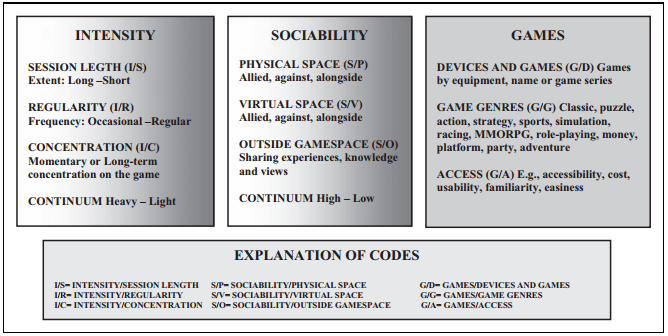
\includegraphics[width=\textwidth]{Figures/kallio-gaming-mentalities-model}
	\caption{The three components of gaming mentalities, as seen in Kallio et al. \cite{kallio2011gamermentalities}}
	\label{fig:kallio-gamer-mentalities-model}
\end{figure}

The social mentality profiles identified by Kallio et al. are of \emph{"quite light"} intensity, very high sociability and their choice in games focus on access to the games. The casual mentality profiles have variable intensity, low sociability and their choice in games focuses primarily on the device and access. The committed mentality profiles have \emph{"heavy"} intensity, high sociability and their choice in games focuses primarily on the genre. Each of the groups of profiles consist of three profiles with different, although similar, values for the various metrics defined in the model. \advice{Is this paragraph (or even source) really of any use here?}

Hamari \& Tuunanen \cite{hamari2014playertypes} used this and other papers to identify a total of five \emph{"key dimensions pertaining to motivations of play/orientation of the player"}: \emph{Achievement}, \emph{Exploration}, \emph{Sociability}, \emph{Domination} and \emph{Immersion}.

In this project, we will use the five archetypal player types \emph{Achieving}, \emph{Exploring}, \emph{Socializing}, \emph{Dominating} and \emph{Immersing}, where each of them is \emph{more concerned with} their respective dimension of the game than the four others, rather than \emph{entirely focused on} only that aspect. That is, for a \emph{Socializing} player, the social aspect of the game is more important than any other aspect, but they may still have varying interest in the other four dimensions.

\todo{Reference these types other places in the report, especially in success factors chapter}

\section{Motivation in Gaming}
\label{sec:motivation-in-gaming}

When considering motivation, we typically distinguish between \emph{intrinsic} and \emph{extrinsic} motivation. \emph{Extrinsic motivation} is motivation from outside sources such as the promise of receiving rewards for successful completion of a task, or punishment should one fail to complete the task. \emph{Intrinsic motivation} on the other hand refers to motivation coming from within, where performing a task is in itself personally rewarding, either because it is fun, exciting, enjoyably challenging or a variety of other positive emotions.

Malone \cite{malone1981toward} proposes challenge, fantasy and curiosity as the primary factors of intrinsic motivation in gaming. Looking back at the player types established in Section \ref{sec:player-types}, the Achieving and Dominating players have challenge as their primary intrinsic motivator, while the Immersing player is motivated by fantasy and the Exploring player is motivated by curiosity. The Socializing player's main source of motivation is not related to the game itself.

While some studies suggest that extrinsic motivation can conflict with and undermine intrinsic motivation (see for example Benabou \& Tirole \cite{benabou2003intrinsic}, Lepper \& Henderlong \cite{lepper2000motivation}), extrinsic rewards are common in video games. By progressing or performing difficult tasks in games, players unlock new types of items or characters, receive powerful items or abilities, in-game currency, cosmetic modifications to their avatar, recognition from other players from being placed in a hall of fame or leader board of some kind, or any number of other rewards. For some, these rewards do indeed remove the fun - the intrinsic motivation - from the game, turning it into a chase for the next reward. For others, however, these rewards help bring back the fun they were no longer able to find, enjoying the game more when being rewarded.

In a market with hundreds of thousands of games and players with short attention spans, however, extrinsic rewards for small feats has become common. To keep players active, they are awarded for doing a minimal amount of effort every day through daily reward systems, often of the form \emph{First X of the day}. For some developers, this is the final step for the game: a last resort to keep players playing their game. For others, it is a means to bridge the gap until they can introduce new features.

\todo{Mention this especially in "reasons to quit - the grind"}

% Chapter - Current state of physical and mental health in society (western world?)
\chapter{Health and Gaming}
\label{chapter:lit-study-modern-health}
\lhead{Chapter \ref{chapter:lit-study-modern-health}. \emph{Modern Society and Health}}

This chapter looks at some previous research on the effect of gaming on physical and mental health.

\section{Physical Activity}
\label{sec:lit-study-physical-activity}

Obesity is becoming an increasing problem as the world is further urbanized, and increasing physical inactivity is an important factor in the trend (Anderson \& Butcher \cite{anderson2006childhood}, Malik et al. \cite{malik2013global}, Uauy et al. \cite{uauy2001obesity}, Wang et al. \cite{wang2011health}). The World Health Organization (WHO) \cite{WHOobesity} report that worldwide obesity has more than doubled since 1980, with 39 \% of adults aged 18 years and older being overweight, and 13 \% being obese. To combat this, they recommend adults do \emph{"at least 150 minutes of moderate-intensity aerobic physical activity throughout the week"}, while children should do 60 minutes per day \cite{WHOphysical}. Janssen \& LeBlanc \cite{janssen2010systematic} performed a review of previous studies on \emph{"the relation between physical activity, fitness, and health in school-aged children and youth"}, and made similar recommendations based on these.

To motivate people to participate in physical activity, an emerging game trend in the last decade have been so-called \emph{exergames}. Whitehead et al. \cite{whitehead2010exergame} describe exergames as \emph{"video games that provide encouragement to exercise, particularly for an audience that may be reluctant to engage in the more traditional forms of exercise"}, further stating that \emph{"Exergames are a commonly accepted method of encouraging more physical activity to promote better health for those with high levels of sedentary screen time"}. Peng et al. \cite{peng2011playing} found that playing exergames were successful in increasing heart rate, oxygen consumption and energy expenditure to levels similar to those of traditional physical activities, and that they can \emph{"facilitate light- to moderate-intensity physical activity promotion"}.

\section{Mental Health}
\label{sec:lit-study-mental-health}

The WHO \cite{WHOdepression} estimate 350 million people worldwide suffering from depression, and the Anxiety and Depression Association of America (ADAA) \cite{ADAAanxiety} reports 18 \% of the US population suffering from anxiety disorders. These are serious disorders, and can in the worst case lead to suicide, yet less than half of those suffering, and in some countries fewer than 10 \% \cite{WHOdepression}, receive treatment for their condition.

Studies show that exercise can have a positive effect on depression, moderately to significantly reducing symptoms (Babyak et al. \cite{babyak2000exercise}, Dunn et al. \cite{dunn2005exercise}, Cooney et al. \cite{cooney2014exercise}), while Petruzzello et al. \cite{petruzzello1991meta}, Salmon \cite{salmon2001effects}, and Ströhle \cite{strohle2009physical} also found potential for a positive effect on anxiety disorders.

Rosenberg et al. \cite{rosenberg2010exergames} found potential for exergames to significantly improve symptoms of depression among elderly, and Brox et al. \cite{brox2011exergames} used exergames to a combined effect of increasing physical activity and decreasing loneliness among elderly.

\todo{Coulton et al. (Harnessing Player Creativity ...) about social in AR games?}


% Chapter - Similar games
\chapter{Similar Games}
\label{chapter:lit-study-similar-games}
\lhead{Chapter \ref{chapter:lit-study-similar-games}. \emph{Game Types}}

This chapter looks at some games that are relevant to compare with Pokémon GO, for the most part miscellaneous pervasive games. Some games are more similar than others, but all of them share some aspect with Pokémon GO, be it the play style, game concepts or the device used to play.

\section{Ingress}

Ingress is a location-aware, augmented reality game for Android and iOS phones. Like Pokémon GO, it was developed by Niantic Labs while it was a part of \emph{Google}. It was first officially released on Android in December 2013, and is considered by many to be the precursor to Pokémon GO. In an interview in October 2013 \cite{gamasutraBadger}, the product manager of Ingress stated that \emph{"Our vision for this, from Niantic Labs, is really to build a platform and to help other game studios, other developers, build similar types of geo-games on top of this infrastructure"}. Not only was it one of the first augmented reality games for mobile devices to enjoy commercial success, but it also laid the groundwork for more games to come. \nice{Maybe something about popularity compared to PoGo}

The game narrative explains that so-called \emph{Exotic Matter (XM)} is spreading across the world from \emph{Portals}, and have been linked to an unseen alien race called \emph{the Shapers}. The players choose between two teams: the \emph{Enlightened}, who embrace the alien influence, and the \emph{Resistance}, who wish to save the human race from their \emph{ingress} into our world. The portals and exotic matter are visible through the player's \emph{scanner}, which is the mobile device the game is installed on.

\begin{figure}[h]
	\centering
	\begin{subfigure}{0.45\textwidth}
		\centering
		
\includegraphics{Figures/ingress-logo}
		\caption{The Ingress logo}
	\end{subfigure}
	~
	\begin{subfigure}{0.45\textwidth}
		\centering
		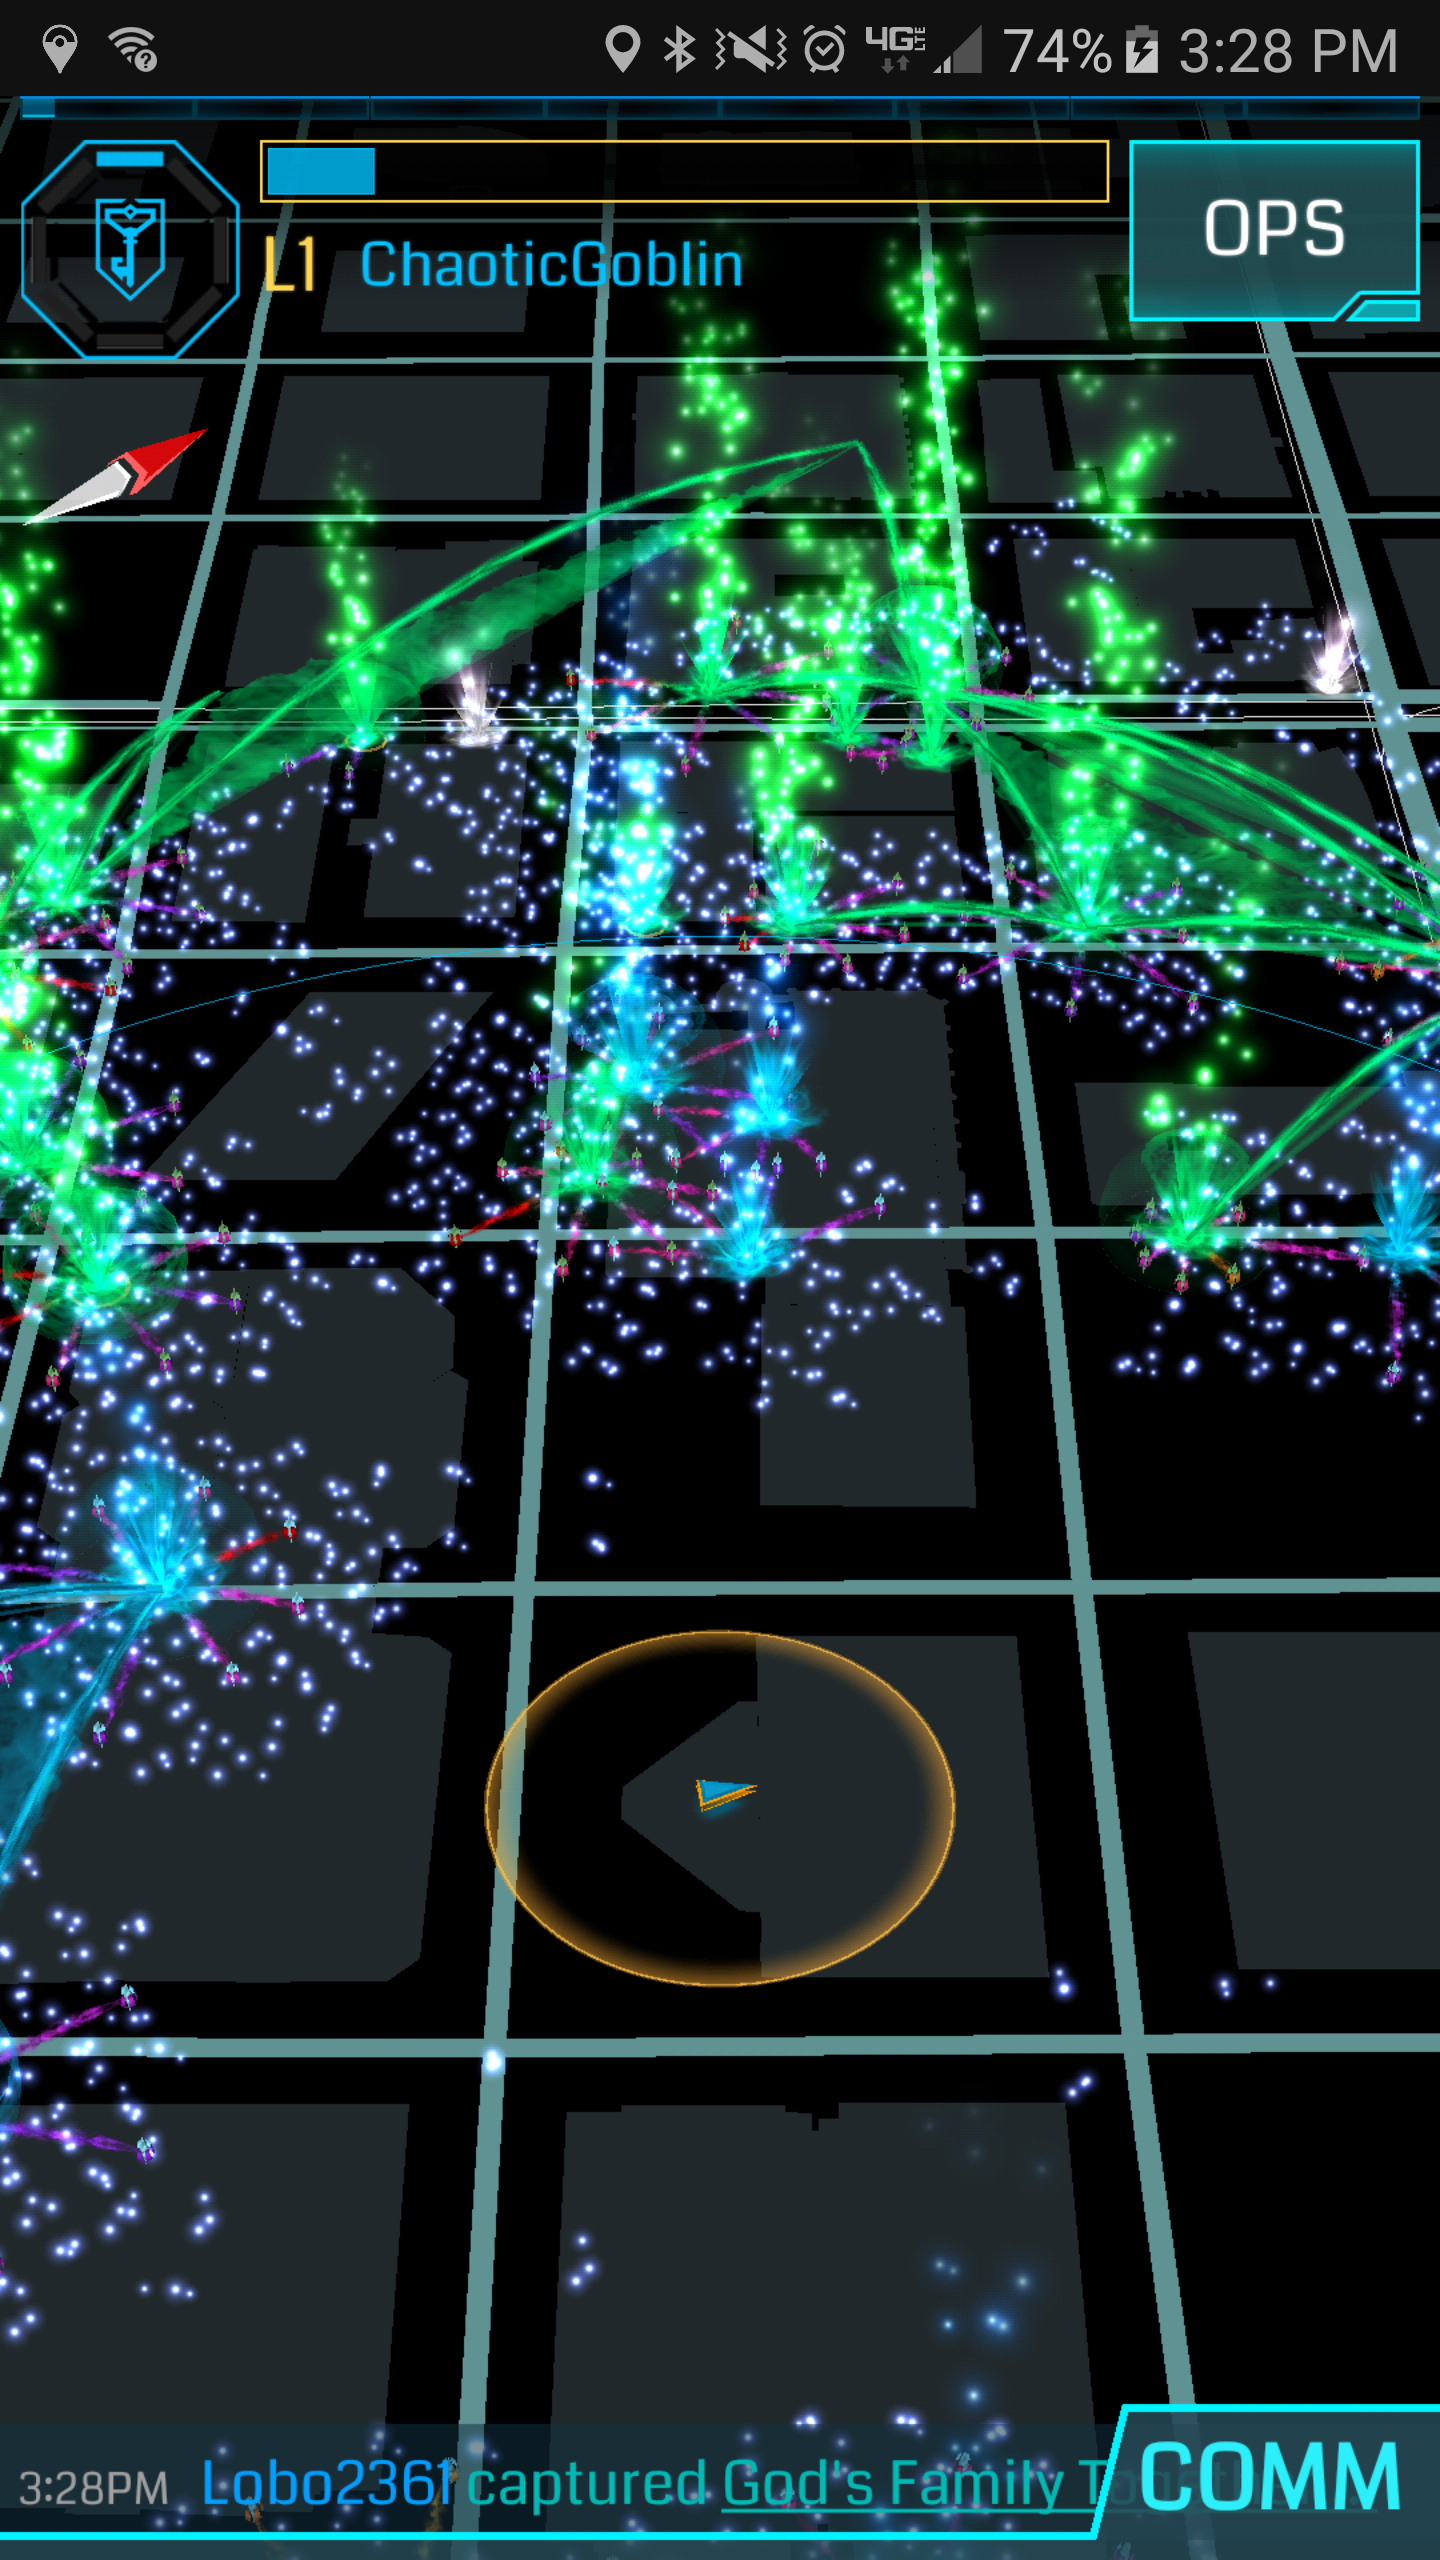
\includegraphics[height=3.2in]{Figures/chaoticgoblin-ingress-screenshot}
		\caption{A screenshot from the game, by Reddit user chaoticgoblin}
	\end{subfigure}
	\caption{Ingress}
\end{figure}

The game revolves around these portals, which players can \emph{hack} to retrieve items that help them claim these and other portals, while the XM they collect by moving around can be used to damage enemy portals. When a team is in complete control of multiple portals, players from that team can \emph{link} these portals to create a \emph{field}. Creating a field will claim the \emph{mind units} under the field for that team.

Portals in the game can be found at landmarks or points of interest, such as statues or buildings of note. Initially, the portals were based on \emph{"historical markers"}, but players could submit locations with descriptions to Niantic, and many of these were added to the game as portals \cite{mashableHanke}. Portal locations were also added later in conjunction with partnerships with various commercial chains such as \emph{Vodafone} \cite{auroraPromotion} or \emph{Jamba Juice}.

Progress in the game comes from performing actions, which yield \emph{action points (AP)} or earning \emph{badges} through achieving specific feats such as holding a friendly portal for a certain amount of time. The rewards for advancing in level is unlocking new, better items, and the only way to advance past level 9 (out of 16) is through earning badges.

Using Kiefer et al.'s \cite{kiefer2006systematically} game dimensions, the game is a \emph{strategy} more than anything else, requiring a solid plan if one wishes to have control over large areas. Although the game is referred to as an augmented reality game, using Kiefer et al.'s definitions, it is closer to a mixed reality game. XM is not perceptible in the real world, nor are the links or fields created. The portals are visible in the real world, but only in the capacity that they are real life objects, and this capacity does not depend on the game. Thus we have to argue that this is a \emph{mixed reality game}. If we ignore the XM, the game is spatially discrete, with game actions only taking place around portals. The collection of XM, however, is spatially continuous, as it can and will be collected mostly anywhere a player goes with the game open. The game is temporally continuous, with actions taking place at any time, although the game restricts the number of actions that can be taken on the same portal in a given time span. \emph{Anomalies}, special events inside and outside the game, take place at specific times, being temporally discrete.

\section{Field Trip}

Another application developed by Niantic is Field Trip. It is not really a game in the way that most people think about games. It does not have rules, goals or other players. It is simply a tool that assists you in exploring. The app encourages you to explore by walking off in any arbitrary direction. When you get close to somewhere interesting, it notifies you. You can set preferences for what type of locations you are interested in, such as \emph{Architecture}, \emph{Historic Places \& Events} or \emph{Cool \& Unique}, and it will ignore other types of places while more frequently notifying you of these types of places.

\begin{figure}[h]
	\centering
	
\includegraphics[width=\textwidth]{Figures/fieldtrip-logo}
	\caption{The Field Trip logo}
\end{figure}

While the application is not a traditional game, it is worth mentioning not only because of its affiliation with Niantic, but because of its integration with Google's augmented reality device \emph{Google Glass}. With Field Trip, the Glasses show you \emph{cards} of the locations you encounter overlaid over what you usually would see, right in front of your eyes without requiring you to look at your phone or a similarly carried device.

Field Trip is also relevant in the way it encourages physical activity by suggesting you walk off in a random direction to explore, rather than find specific places before going out and traveling directly to them, something that often involves less physically exerting modes of transportation. Given that you are exploring somewhere with locations within your field of interest registered in Google's databases, Field Trip rewards you for your (potentially unintended) exercise with new, possibly exciting locations. These features resemble those of some exergames, motivating "players" to exercise through untraditional means.

\section{Geocaching}

Geocaching is a popular family activity game similar to the sport \emph{orienteering}. It is a game played with real life objects, but uses a mobile application to register the location of the items. The application lets you see a map of caches in an area, register your findings and make lists for a planned session. The caches are objects placed at any location, and are typically hidden somewhere clever in this location. The objects are usually minor trinkets intended to be found and then hid again, but some players choose to hide small treasures for the finder to keep. Some caches require that you solve puzzles in the app before its exact coordinates are revealed to you.

\begin{figure}[h]
	\centering
	\begin{subfigure}[t]{0.5\textwidth}
		
\includegraphics[height=2.5in]{Figures/chaoticgoblin-geocache-covered}
		\caption{Cache covered in natural camouflage}
	\end{subfigure}
	~
	\begin{subfigure}[t]{0.4\textwidth}
		
\includegraphics[height=2.5in]{Figures/chaoticgoblin-geocache-birdhouse}
		\caption{Cache hidden in birdhouse}
	\end{subfigure}
	~
	\begin{subfigure}[t]{\textwidth}
		\centering
		
\includegraphics[height=2.5in]{Figures/chaoticgoblin-geocache-camo}
		\caption{Cache in camouflage-taped container}
	\end{subfigure}
	\caption{Clever hiding spots for geocaches (by Reddit user chaoticgoblin)}
	\label{fig:geocache-spots}
\end{figure}

Going back to Kiefer et al.'s \cite{kiefer2006systematically} dimensions for location-based games, Geocaching is primarily an item hunt game, and is in fact used as the most prominent example of one in their paper. Figure \ref{fig:geocache-spots} shows three clever hiding spots for caches found by Reddit user \emph{chaoticgoblin}, intended to make the player really have to search to find them. However, with the addition of caches that require you to solve puzzles to reveal their coordinates, Geocaching also gains aspects of a puzzle game. It is a pure location-based game, using localization technology solely to inform players of the location of the physical items, items that have no virtual equivalent. While caches technically can be placed anywhere, the actual locations of caches, where game events take place, are discrete and fairly static. Creating and placing a new cache can be done anywhere, but once placed, the location is discrete. Thus we classify Geocaching as spatially discrete. The game can be played at any time, and is thus temporally continuous.

\section{Zombies, Run!}

Zombies, Run! is an exergame for Android and iOS devices. First released in 2012, it has added a new \emph{season} of content each year since, and now has 200 missions to play through. Within two weeks of its release, it was the highest grossing app in the Health \& Fitness category in the iOS App Store, and now has a million players.

\begin{figure}[h]
	\centering
	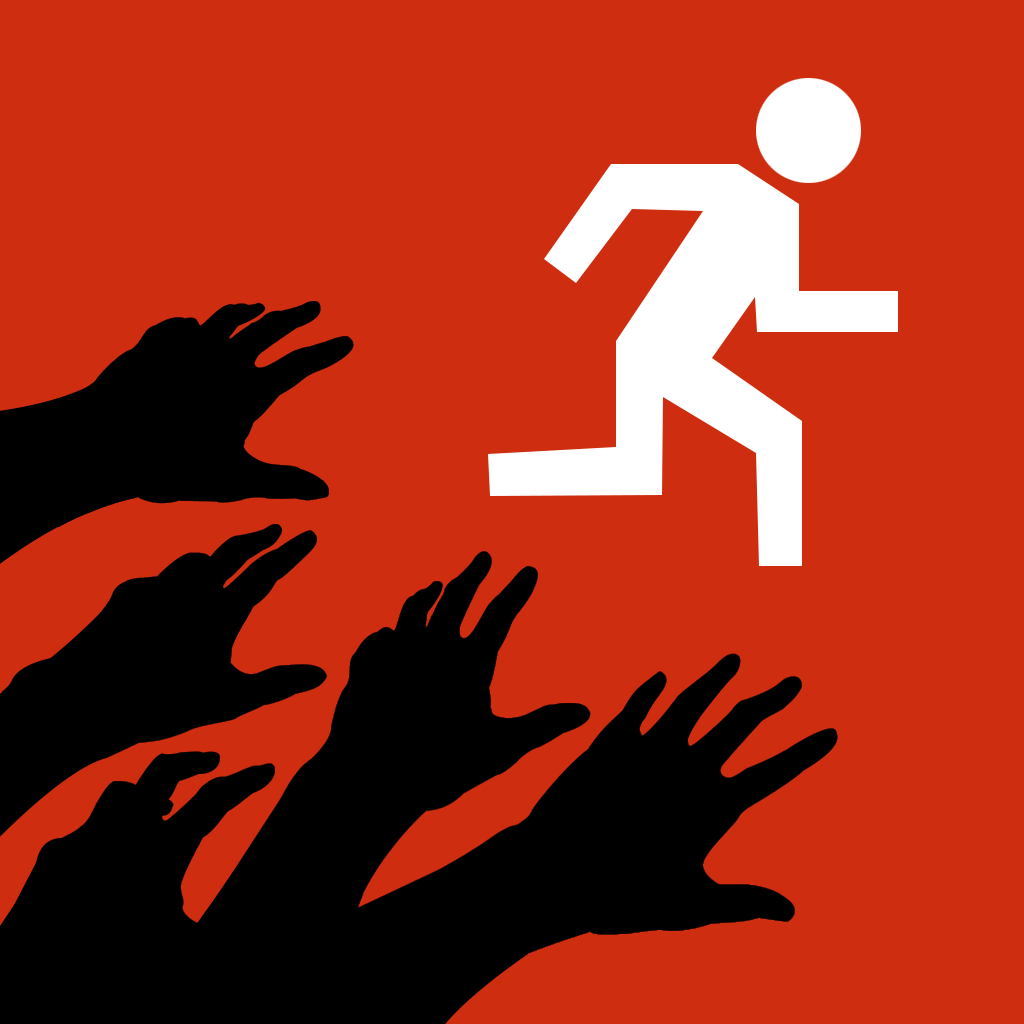
\includegraphics[height=2in]{Figures/zombies-run-logo}
	\caption{The \emph{Zombies, Run!} logo}
\end{figure}

The game narrative places the player in a post-zombie-apocalyptic world, and you are one of few survivors. By going out to run, you'll collect supplies used to build up a base for you and fellow survivors. The game features 200 missions that are narrated mini-stories that drive the plot forward as you build up your base, playing audio clips in between your own music as you run. During your run, it is possible for zombies to appear and chase you, requiring an increased pace. Should you fail to increase your pace and outrun them, they will catch up to you and any supplies you have collected will be lost.

The game uses the device screen minimally to select missions and viewing and sharing your progress between runs, while the game experience is presented through audio. There are no visual augmentations of reality, but the game uses audio clips to perceptibly augment a run. When being chased by zombies, their groans can be heard closing in if you do not run quickly enough, and their distance to you can be felt through the volume and intensity of their sounds. The game also plays a heartbeat in your ears, intended to imitate your own as you run. Southerton \cite{southerton2013zombies} performed an \emph{autoethnography} noting her experiences with the game, and found the heartbeat in particular to add high levels of immersion by adding a sense of urgency, but only during the other audio clips presented by the game.

\begin{figure}[h]
	\centering
	\begin{subfigure}{0.45\textwidth}
		\centering
		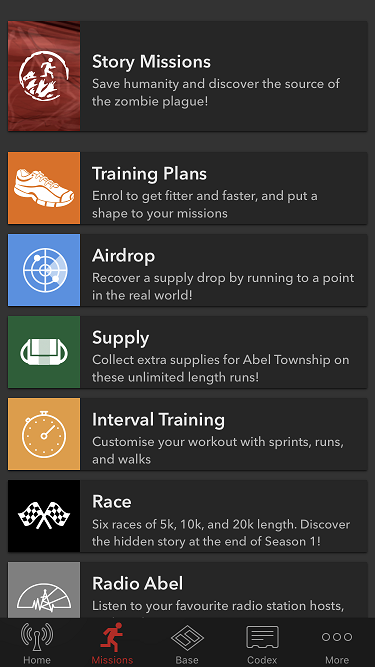
\includegraphics[height=3in]{Figures/zombies-run-activities}
		\caption{Activities available}
	\end{subfigure}
	~
	\begin{subfigure}{0.45\textwidth}
		\centering
		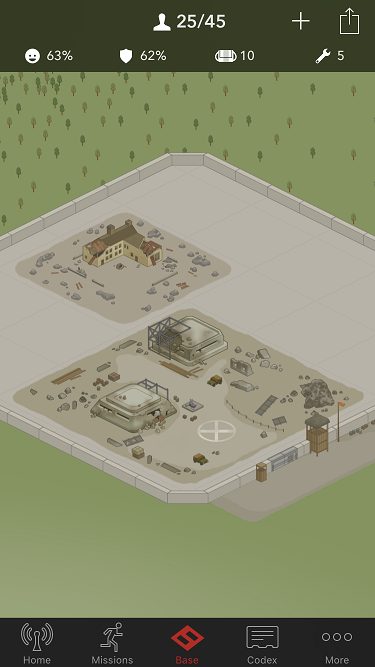
\includegraphics[height=3in]{Figures/zombies-run-base}
		\caption{View of the player's base}
	\end{subfigure}
	\caption{Screenshots of \emph{Zombies, Run!}}
\end{figure}

With basis in Kiefer et al.'s \cite{kiefer2006systematically} paper, Zombies, Run! is a location-based game in that it uses GPS technology to track the player's movements in order to progress in the game by collecting supplies and to escape zombies. It also allows the player to choose a location on a map, and will generate a mission tailored to the distance to that location, called an \emph{Airdrop}. We classify Zombies, Run! as an augmented reality game, with virtual elements (zombies) perceptible in the real world through audio. The game is closest to a chase game, as outrunning the zombies is vital to game progress. The game progresses continually as the player moves, as long as they are on a mission, and a mission can be started at any time. Thus we classify the game as spatially and temporally continuous.

While the game is an exergame in the true sense of being a game with the sole purpose of encouraging physical activity, or more specifically aerobic exercise, the actual impact of the exercise it encourages has been debated. Halushak, an experienced runner, noted in her experience with the game that because of the sparse zombie attacks and high requirement to escape them that the game is more about exercising the players' imagination than to push them to their limits. Halushak's reasoning for this is that the player must increase their pace by at least 20 \% to escape, which is difficult when already running at a quick pace, encouraging an overall lower pace if one wants to be able to escape. Higgins \cite{higgins2016smartphone} in a review of smartphone apps for increasing patients' health and fitness recommended the game for \emph{"healthy patients wanting to start basic aerobic exercise"}, but not any other groups of patients. Other studies (Cowdery et al. \cite{cowdery2015exergame} and Direito et al. \cite{direito2015apps}) performed with the app showed that the physical impact was limited, but that players using these apps were more likely to be motivated to continue their exercise after the control periods.

\section{Munzee}
\todo{Exergame}

\section{Stolpejakten}
\todo{Exergame}

\section{Run an Empire}
\todo{Exergame}

\section{The Walk}
\todo{Story-driven audio AR}

\section{Mobile games}
\todo{Some examples of casual mobile games (e.g. Angry Birds, Candy Crush, Temple Run)}


% Chapter - More about Pokémon and Pokémon GO
\chapter{Pokémon}
\label{chapter:lit-study-pokemon-go}
\lhead{Chapter \ref{chapter:lit-study-pokemon-go}. \emph{Pokémon GO}}

\section{Pokémon Franchise}
\todo{Short introduction to the Pokémon franchise, some terms and the different games?}

\section{Pokémon GO In-Depth}
\label{sec:pokemon-go-in-depth}
\todo{Description of every feature of Pokémon GO, and the technology it uses. Also describe game type based on theory from Chapter \ref{chapter:lit-study-game-theory}}

\section{Pokémon GO in the Media}
\todo{Mention and cite some articles about Pokémon GO. } \advice{Are Norwegian articles fine?}
